\documentclass[tikz, border=4pt]{standalone}
\usepackage{tikz}
\usepackage{pgfplots}
\pgfplotsset{compat=1.18}
\begin{document}
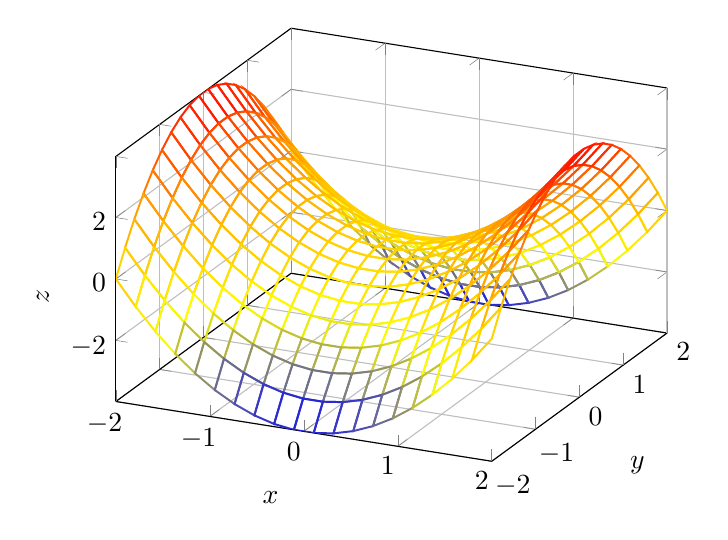
\begin{tikzpicture}[x=1cm, y=1cm]
  \definecolor{tdc1}{HTML}{1E5BD6}

  \begin{axis}[
    at={(0cm,-5.5cm)},
    anchor=south west,
    scale only axis,
    width=7cm,
    height=5.5cm,
    xmin=-2,
    xmax=2,
    ymin=-2,
    ymax=2,
    zmin=-3.9889,
    zmax=3.9889,
    view={25}{30},
    xtick={-2,-1,0,1,2},
    ytick={-2,-1,0,1,2},
    ztick={-2,0,2},
    grid=major,
    xlabel={$x$},
    ylabel={$y$},
    zlabel={$z$},
    colormap={tdmap}{rgb255(0cm)=(0,0,255); rgb255(1cm)=(255,255,0); rgb255(2cm)=(255,165,0); rgb255(3cm)=(255,0,0)},
    point meta min=-3.9889,
    point meta max=3.9889
  ]
    \addplot3[mesh, line width=0.71pt, domain=-2:2, y domain=-2:2, samples=20, forget plot] {((x)^(2)-(y)^(2))};
  \end{axis}
\end{tikzpicture}
\end{document}
